\documentclass[conference]{IEEEtran}
\IEEEoverridecommandlockouts
\usepackage{cite}
\usepackage{amsmath,amssymb,amsfonts}
\usepackage{graphicx}
\graphicspath{{figures/}}
\usepackage{textcomp}
\usepackage{xcolor}
\usepackage{booktabs}
\usepackage{hyperref}
\usepackage{tikz}
\usetikzlibrary{positioning,fit,backgrounds,arrows.meta}
\newcommand{\softred}[1]{\textcolor{red!70!black}{#1}}
\newcommand{\softgreen}[1]{\textcolor{green!60!black}{#1}}
\def\BibTeX{{\rm B\kern-.05em{\sc i\kern-.025em b}\kern-.08em
    T\kern-.1667em\lower.7ex\hbox{E}\kern-.125emX}}

\begin{document}

\title{RoadFury at the ICST 2026 Tool Competition --\\Self-Driving Car Testing Track}

\author{
\IEEEauthorblockN{
Chi-Nguyen Tran$^*$,
Dao Sy Duy Minh$^*$,
Huynh Trung Kiet$^*$,
Phu-Hoa Pham,
Nguyen Lam Phu Quy
}
\IEEEauthorblockA{\textit{Faculty of Information Technology, University of Science (HCMUS), Vietnam}}
\IEEEauthorblockA{\textit{Vietnam National University -- Ho Chi Minh City (VNU-HCM), Vietnam}}
\IEEEauthorblockA{\{23122044, 23122041, 23122039, 23122030, 23122048\}@student.hcmus.edu.vn}
\IEEEauthorblockA{$^*$Equal contribution}
}
\maketitle

\begin{abstract}
We present \textbf{RoadFury}, a test prioritization tool for the ICST~2026 SDC Testing Competition~\cite{b8}.
Existing approaches reduce road geometry to aggregate statistics, discarding the sequential structure that makes roads dangerous.
RoadFury instead preserves the full geometric sequence: a 10-channel feature matrix encoding curvature, heading, jerk, and positional context at every road point, processed by a Pre-LN Transformer Encoder~\cite{b11} stabilized with Stochastic Weight Averaging (SWA)~\cite{b6}.
Deployed as a Docker-containerized gRPC service, RoadFury achieves APFD~=~\textbf{0.804\,$\pm$\,0.012}, surpassing the prior best of 0.781 and outperforming LLM, GNN, and CNN baselines.
\end{abstract}

\begin{IEEEkeywords}
test prioritization, self-driving cars, Transformer, stochastic weight averaging
\end{IEEEkeywords}

%=====================================================================
\section{Introduction}

Testing self-driving cars (SDCs) in simulators such as BeamNG.tech is essential yet expensive~\cite{b1,b2}.
\emph{Test prioritization} reorders a test suite so that failure-revealing cases execute first, maximizing early fault detection.
The standard metric is APFD~\cite{b4}:
\begin{equation}
\text{APFD}(\pi) = 1 - \frac{\sum_{i=1}^{m} TF_i}{n \cdot m} + \frac{1}{2n},
\end{equation}
where $n$ is the total number of tests, $m$ the number of failing tests, and $TF_i$ the rank of the $i$-th fault in ordering $\pi$.
A higher APFD indicates that faults are exposed earlier in the execution.

Existing tools such as SDC-Scissor~\cite{b1,b2} summarize each road by three aggregate statistics (mean curvature, mean lateral position, standard deviation) and feed them into a feedforward network.
This representation collapses the \emph{ordered sequence} of road geometry into a fixed-size vector, discarding spatial transitions---consecutive sharp bends, sudden jerk changes---that most reliably predict SDC failures.
\textbf{RoadFury} treats each road as a full sequence and learns over it with a Pre-LN Transformer Encoder~\cite{b11} regularized by SWA~\cite{b6}.

\section{Approach}

\subsection{Feature Extraction}

Each test case is defined by a variable-length sequence of 2D road control points.
We uniformly resample every road to $L{=}197$ points and compute 10 intrinsic geometry channels at each point (Table~\ref{tab:features}), yielding a $(197{\times}10)$ feature matrix that is translation- and rotation-invariant.
All channels are z-normalized using per-channel mean and standard deviation computed on the training set.

\begin{table}[t]
\caption{10-Channel Road Geometry Feature Set}
\vspace{-4pt}
\begin{center}
\setlength{\tabcolsep}{3pt}
{\small\begin{tabular}{cll}
\toprule
\textbf{Ch.} & \textbf{Feature} & \textbf{Definition} \\
\midrule
$f_0$ & Segment length      & $\|p_{i+1}-p_i\|_2$ \\
$f_1$ & Abs.\ angle change  & $|\Delta\theta_i|$ \\
$f_2$ & Menger curvature    & $\kappa_i=4A_i/(a_i b_i c_i)$ \\
$f_3$ & Curvature jerk      & $\Delta\kappa_i$ \\
$f_4$ & Cum.\ dist.\ norm   & $\sum\|p_{j+1}{-}p_j\|/d_\text{tot}$ \\
$f_5$ & Heading $\sin$      & $\sin(\theta_i)$ \\
$f_6$ & Heading $\cos$      & $\cos(\theta_i)$ \\
$f_7$ & Rel.\ position      & $i/(L{-}1)\in[0,1]$ \\
$f_8$ & Local curv.\ std    & $\text{std}(\kappa_{i-5{:}i+5})$ \\
$f_9$ & Curv.\ acceleration & $\Delta^2\kappa_i$ \\
\bottomrule
\end{tabular}}
\label{tab:features}
\end{center}
\vspace{-6pt}
\end{table}

\subsection{RoadTransformer Architecture}

\begin{figure*}[t]
\centering
\resizebox{0.54\textwidth}{!}{%
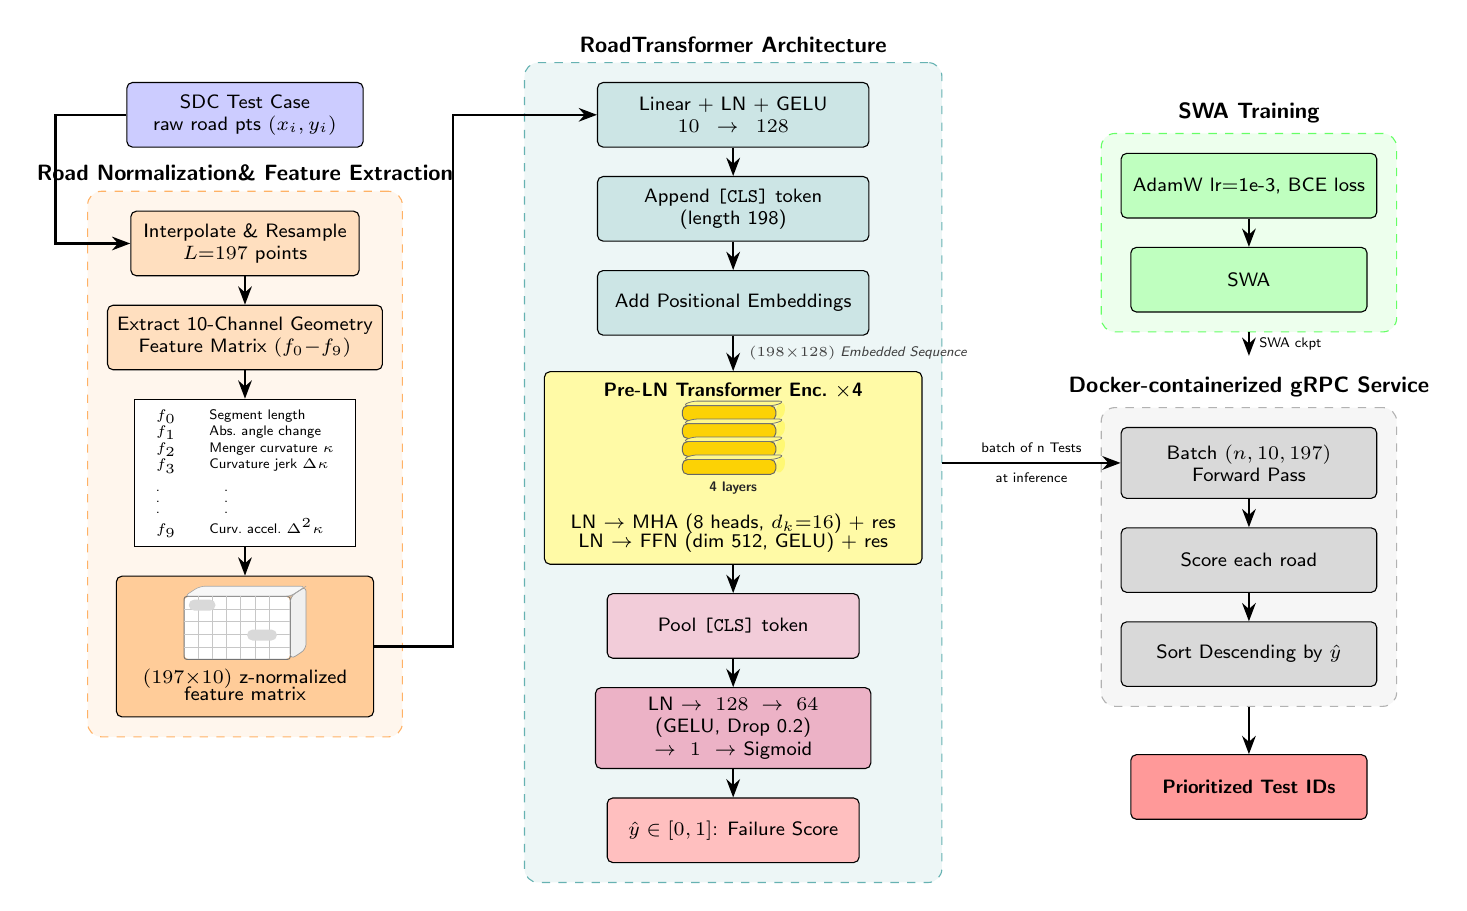
\begin{tikzpicture}[
  font=\sffamily\scriptsize,
  >=Stealth,
  node distance=0.36cm,
  arr/.style={->, thick},
  blk/.style={draw, rounded corners=2pt, fill=#1, align=center,
              inner sep=3.5pt, minimum width=2.9cm, minimum height=0.82cm},
  grp/.style={draw=#1!60, dashed, rounded corners=5pt,
              inner sep=7pt, fill=#1!7},
  htitle/.style={font=\sffamily\bfseries\footnotesize},
]

%% ===== LEFT: INPUT & FEATURE EXTRACTION =====

\node[blk=blue!20, minimum width=3.0cm] (sdc) at (0,0)
    {SDC Test Case\\raw road pts $(x_i, y_i)$};

\node[blk=orange!25, below=0.80cm of sdc] (resamp)
    {Interpolate \& Resample\\$L{=}197$ points};

\node[blk=orange!25, below=0.36cm of resamp] (feat)
    {Extract 10-Channel Geometry\\Feature Matrix $(f_0{-}f_9)$};

\node[draw, fill=white, inner sep=3pt, below=0.36cm of feat,
      font=\sffamily\tiny, minimum width=2.8cm] (ftab)
    {\begin{tabular}{@{}ll@{}}
       $f_0$ & Segment length \\
       $f_1$ & Abs.\ angle change \\
       $f_2$ & Menger curvature $\kappa$ \\
       $f_3$ & Curvature jerk $\Delta\kappa$ \\
       $\vdots$ & \quad $\vdots$ \\
       $f_9$ & Curv.\ accel.\ $\Delta^2\kappa$ \\
     \end{tabular}};

\node[blk=orange!40, below=0.36cm of ftab, minimum width=3.0cm] (znorm)
    {\begin{tabular}{c}
      \tikz[baseline=-0.6ex]{
        % 3D CNN-style slanted feature "matrix" block
        \def\w{1.35}  % front width (bigger)
        \def\h{0.80}  % front height (taller)
        \def\dx{0.20} % depth x-shift
        \def\dy{0.13} % depth y-shift
        % faces
        \fill[white] (0,0) rectangle (\w,\h);
        \fill[black!6] (\w,0) -- (\w,\h) -- (\w+\dx,\h+\dy) -- (\w+\dx,\dy) -- cycle; % right
        \fill[black!3] (0,\h) -- (\w,\h) -- (\w+\dx,\h+\dy) -- (\dx,\h+\dy) -- cycle; % top
        % outline
        \draw[black!55, line width=0.35pt, rounded corners=1.0pt] (0,0) rectangle (\w,\h);
        \draw[black!40, line width=0.25pt] (\w,0) -- (\w,\h) -- (\w+\dx,\h+\dy) -- (\w+\dx,\dy) -- cycle;
        \draw[black!35, line width=0.22pt] (0,\h) -- (\w,\h) -- (\w+\dx,\h+\dy) -- (\dx,\h+\dy) -- cycle;
        \draw[black!35, line width=0.22pt] (\w,\h) -- (\w+\dx,\h+\dy);
        % front-face grid
        \foreach \x in {0.18,0.36,...,1.26} \draw[black!22, line width=0.20pt] (\x,0) -- (\x,\h);
        \foreach \y in {0.16,0.32,...,0.80} \draw[black!22, line width=0.20pt] (0,\y) -- (\w,\y);
        % small "activations" on the front face
        \fill[black!15] (0.06,0.62) rectangle (0.40,0.76);
        \fill[black!15] (0.80,0.24) rectangle (1.18,0.38);
      }\\[-1pt]
      {\scriptsize $(197{\times}10)$ z-normalized}\\[-2pt]
      {\scriptsize feature matrix}
    \end{tabular}};

\begin{pgfonlayer}{background}
  \node[grp=orange, fit=(resamp)(feat)(ftab)(znorm),
        label={[htitle]above=2pt:Road Normalization\\\& Feature Extraction}] (leftgrp) {};
\end{pgfonlayer}

%% ===== MIDDLE: ROADTRANSFORMER ARCHITECTURE =====

\node[blk=teal!20, minimum width=3.2cm, text width=3.2cm] (proj) at (6.2,0)
    {Linear + LN + GELU\\$10 \to 128$};

\node[blk=teal!20, minimum width=3.2cm, text width=3.2cm, below=0.36cm of proj] (cls)
    {Append \texttt{[CLS]} token\\(length 198)};

\node[blk=teal!20, minimum width=3.2cm, text width=3.2cm, below=0.36cm of cls] (posemb)
    {Add Positional Embeddings};

\node[blk=yellow!35, minimum width=3.3cm, minimum height=1.35cm,
      below=0.45cm of posemb] (enc)
    {\begin{tabular}{c}
      \textbf{Pre-LN Transformer Enc.\ $\times$4}\\[-1pt]
      \raisebox{-2pt}{\tikz[baseline=-0.6ex, scale=0.95]{
        % PlotNeuralNet-style 3D cuboid stack (4 layers)
        \def\xL{0.00} \def\xR{1.25}
        \def\hF{0.20} \def\step{0.24}
        \def\dx{0.12} \def\dy{0.06}
        % Draw back-to-front for proper overlap
        \foreach \i in {3,2,1,0} {
          \pgfmathsetmacro{\yB}{0.02+\i*\step}
          \pgfmathsetmacro{\yT}{\yB+\hF}
          % right face
          \fill[yellow!55!white]
            (\xR,\yB) -- (\xR,\yT) -- (\xR+\dx,\yT+\dy) -- (\xR+\dx,\yB+\dy) -- cycle;
          % front face
          \fill[yellow!70!orange]
            (\xL,\yB) rectangle (\xR,\yT);
          \draw[black!60, line width=0.35pt]
            (\xL,\yB) rectangle (\xR,\yT);
          % top face
          \fill[yellow!45!white]
            (\xL,\yT) -- (\xR,\yT) -- (\xR+\dx,\yT+\dy) -- (\xL+\dx,\yT+\dy) -- cycle;
          \draw[black!55, line width=0.28pt]
            (\xL,\yT) -- (\xR,\yT) -- (\xR+\dx,\yT+\dy) -- (\xL+\dx,\yT+\dy) -- cycle;
        }
        \node[font=\sffamily\tiny\bfseries, text=black!85] at (0.68,0.55) {4 layers};
      }}\\[-10pt]
      \raisebox{3pt}{{\scriptsize LN $\rightarrow$ MHA (8 heads, $d_k{=}16$) + res}}\\[-4pt]
      {\scriptsize LN $\rightarrow$ FFN (dim 512, GELU) + res}
    \end{tabular}};

\node[blk=purple!20, minimum width=3.2cm, below=0.36cm of enc] (pool)
    {Pool \texttt{[CLS]} token};

\node[blk=purple!30, minimum width=3.2cm, text width=3.25cm,
      below=0.36cm of pool, minimum height=0.95cm] (mlp)
    {LN $\to 128 \to 64$\\(GELU, Drop 0.2)\\$\to 1 \to$ Sigmoid};

\node[blk=red!25, minimum width=3.2cm, below=0.36cm of mlp] (yhat)
    {$\hat{y} \in [0,1]$: Failure Score};

\begin{pgfonlayer}{background}
  \node[grp=teal,
        fit=(proj)(cls)(posemb)(enc)(pool)(mlp)(yhat),
        label={[htitle]above:RoadTransformer Architecture}] (midgrp) {};
\end{pgfonlayer}

%% ===== RIGHT: DEPLOYMENT =====

\node[blk=green!25, minimum width=3.0cm, text width=3.0cm] (adam) at (12.75, -0.9)
    {AdamW lr$=$1e-3, BCE loss};

\node[blk=green!25, minimum width=3.0cm, below=0.36cm of adam] (swabox)
    {SWA};

\begin{pgfonlayer}{background}
  \node[grp=green, fit=(adam)(swabox),
        label={[htitle]above:SWA Training}] (swagrp) {};
\end{pgfonlayer}

\node[blk=gray!30, minimum width=3.0cm, text width=3.0cm,
      below=1.20cm of swagrp.south, minimum height=0.90cm] (bfwd)
    {Batch $(n,10,197)$\\Forward Pass};

\node[blk=gray!30, minimum width=3.0cm, text width=3.0cm,
      below=0.36cm of bfwd, minimum height=0.82cm] (scorerd)
    {Score each road};

\node[blk=gray!30, minimum width=3.0cm, text width=3.0cm,
      below=0.36cm of scorerd, minimum height=0.82cm] (sortd)
    {Sort Descending by $\hat{y}$};

\begin{pgfonlayer}{background}
  \node[grp=gray, fit=(bfwd)(scorerd)(sortd),
        label={[htitle]above:Docker-containerized gRPC Service}] (dkgrp) {};
\end{pgfonlayer}

\node[blk=red!40, minimum width=3.0cm, below=0.6cm of dkgrp.south] (result)
    {\textbf{Prioritized Test IDs}};

%% ===== ARROWS =====

% Left internal
\draw[arr] (sdc.west) -- ++(-0.9,0) |- (resamp.west);
\draw[arr] (resamp) -- (feat);
\draw[arr] (feat)   -- (ftab);
\draw[arr] (ftab)   -- (znorm);

% Left → Middle
\draw[arr] (znorm.east) -- ++(1.00,0) |- (proj.west);

% Middle internal
\draw[arr] (proj)   -- (cls);
\draw[arr] (cls)    -- (posemb);
\draw[arr] (posemb) -- node[midway, right=2pt, font=\sffamily\tiny\itshape, text=black!75] {$(198{\times}128)$ Embedded Sequence} (enc);
\draw[arr] (enc)    -- (pool);
\draw[arr] (pool)   -- (mlp);
\draw[arr] (mlp)    -- (yhat);

% Right internal
\coordinate (dktitle) at ([yshift=0.65cm]dkgrp.north);
% AdamW -> SWA (SWA tracks averaged weights)
\draw[arr] (adam.south) -- (swabox.north);
\draw[arr] (swagrp.south) -- node[midway, right, font=\sffamily\tiny] {SWA ckpt} (dktitle);
\draw[arr] (bfwd)    -- (scorerd);
\draw[arr] (scorerd) -- (sortd);
\draw[arr] (dkgrp.south) -- (result);

% Middle → Right: inference path (RoadTransformer → Docker)
\draw[arr] (midgrp.east |- bfwd.west) -- (bfwd.west)
    node[midway, above, font=\sffamily\tiny] {batch of n Tests}
    node[midway, below, font=\sffamily\tiny] {at inference};

\end{tikzpicture}%
}
\caption{RoadFury pipeline: (1)~road control points are uniformly resampled; (2)~10 geometry channels are extracted per point; (3)~a Pre-LN Transformer Encoder with a \texttt{[CLS]} token produces a failure score $\hat{y}$; the model is trained with SWA and served as a Docker gRPC service that returns prioritized test IDs.}
\label{fig:arch}
\end{figure*}

Fig.~\ref{fig:arch} illustrates the complete pipeline.
A linear projection maps each 10-dim point vector to a 128-dim embedding, followed by LayerNorm and GELU activation.
A learnable \texttt{[CLS]} token is prepended to the sequence and sinusoidal positional embeddings are added, yielding 198 tokens in total.
A 4-layer Pre-LN Transformer Encoder~\cite{b11} ($d{=}128$, 8~heads, FFN width 512, dropout 0.1) then applies global self-attention over the entire road trajectory.
The resulting \texttt{[CLS]} representation passes through a two-layer MLP head (GELU activations, dropout) to produce a failure probability $\hat{y}$, which is used to rank tests in descending order.
The model has 829K parameters in total.

\subsection{Training and Deployment}

We train on 28,804 labeled road--outcome pairs from SensoDat~\cite{b7} using AdamW (lr$=$5$\times$10$^{-4}$, weight~decay$=$10$^{-3}$) with binary cross-entropy loss for 75 epochs.
SWA~\cite{b6} collects weight snapshots from epochs 50--75 and averages them, yielding a flatter loss landscape and improved generalization.
The trained model is packaged as a Docker-containerized gRPC microservice exposing three endpoints: \texttt{Name}, \texttt{Initialize}, and \texttt{Prioritize}.

\section{Evaluation}

\subsection{Results}

We evaluate on the 956-test competition set~\cite{b8}, averaging APFD over 30 independent random trials to account for tie-breaking variance in the ranking.
Table~\ref{tab:results} compares RoadFury against four alternative paradigms explored during development.

\begin{table}[t]
\caption{Multi-Paradigm Comparison (956 competition tests, 30 trials)}
\vspace{-4pt}
\begin{center}{\small
\setlength{\tabcolsep}{3pt}
\begin{tabular}{lcc}
\toprule
\textbf{Method} & \textbf{APFD} & \textbf{Paradigm} \\
\midrule
Random                   & 0.493              & -- \\
LLM zero-shot            & 0.487\,$\pm$\,0.019 & Language model \\
GNN (road graph)         & 0.533\,$\pm$\,0.025 & 3-layer GCN~\cite{b10} \\
ResNet-50 visual         & 0.572\,$\pm$\,0.013 & Road image CNN \\
ITEP4SDC                 & 0.781              & MLP, 3 features \\
\textbf{RoadFury (ours)} & \textbf{0.804\,$\pm$\,0.012} & \textbf{Transformer+SWA} \\
\bottomrule
\end{tabular}}
\label{tab:results}
\end{center}
\vspace{-6pt}
\end{table}

RoadFury outperforms all baselines.
LLMs reason over natural-language road descriptions and miss fine-grained numeric geometry; GNNs capture pairwise adjacency but lose the ordered trajectory dynamics; CNNs applied to road images sacrifice the numeric precision of curvature values.
RoadFury's Transformer attends directly over ordered curvature transitions, capturing the spatial patterns most predictive of simulation failures.

\subsection{Ablation}

Table~\ref{tab:ablation} reports the effect of seven modifications applied independently to the base RoadTransformer trained without SWA.
All numbers are averaged over 30 trials on the 956-test competition set.

\begin{table}[t]
\caption{Ablation Study (956 competition tests, 30 trials)}
\vspace{-4pt}
\begin{center}{\small
\setlength{\tabcolsep}{3pt}
\begin{tabular}{lc}
\toprule
\textbf{Modification} & \textbf{APFD} \\
\midrule
RoadTransformer (no SWA)        & 0.788\,$\pm$\,0.014 \\
\midrule
+~Multi-scale Conv Stem         & \softred{0.767\,$\pm$\,0.014~$\downarrow$} \\
+~Stochastic Depth (DropPath)   & \softred{0.768\,$\pm$\,0.015~$\downarrow$} \\
+~Triple Pooling (CLS+Mean+Max) & \softred{0.768\,$\pm$\,0.015~$\downarrow$} \\
+~Mixup augmentation            & \softred{0.773\,$\pm$\,0.015~$\downarrow$} \\
+~Focal Loss ($\gamma{=}2$)~\cite{b9} & \softred{0.782\,$\pm$\,0.014~$\downarrow$} \\
+~Test-time augmentation (TTA)  & \softred{0.770\,$\pm$\,0.016~$\downarrow$} \\
\textbf{+~SWA}                  & \textbf{\softgreen{0.804\,$\pm$\,0.012~$\uparrow$}} \\
\bottomrule
\end{tabular}}
\label{tab:ablation}
\end{center}
\vspace{-6pt}
\end{table}

Every modification except SWA degraded or matched base performance.
SWA is the only one that consistently improved APFD, confirming that weight averaging over flat optima matters more than architectural changes or data augmentation.

\section{Conclusion}

Preserving sequential road geometry, rather than aggregating it, is the key to effective SDC test prioritization.
A Pre-LN Transformer with SWA achieves APFD\,=\,0.804\,$\pm$\,0.012, the best result in the ICST~2026 SDC Testing Competition.
We plan to investigate richer simulation feedback signals and cross-simulator transfer.
The tool is publicly available at \url{https://github.com/chisngyen/sdc-test-prioritization-novel}.

{\small
\vspace{-5pt}
\begin{thebibliography}{00}
\bibitem{b1} C. Birchler, S. Khatiri, B. Bosshard, A. Gambi, and S. Panichella, ``Machine learning-based test selection for simulation-based testing of self-driving cars software,'' \textit{Empir. Softw. Eng.}, vol.~28, no.~71, 2023.
\bibitem{b2} C. Birchler, N. Ganz, S. Khatiri, A. Gambi, and S. Panichella, ``Cost-effective simulation-based test selection in self-driving cars software with SDC-Scissor,'' in \textit{Proc. IEEE SANER}, 2022, pp.~386--390.
\bibitem{b4} S. Yoo and M. Harman, ``Regression testing minimization, selection and prioritization: A survey,'' \textit{Softw. Test. Verif. Reliab.}, vol.~22, no.~2, pp.~67--120, 2012.
\bibitem{b6} P. Izmailov, D. Podoprikhin, T. Garipov, D. Vetrov, and A. G. Wilson, ``Averaging weights leads to wider optima and better generalization,'' in \textit{Proc. UAI}, 2018.
\bibitem{b7} C. Birchler, S. Khatiri, C. Rohrbach, T. Kehrer, and S. Panichella, ``SensoDat: Simulation-based sensor dataset of self-driving cars,'' in \textit{Proc. IEEE/ACM MSR}, 2024.
\bibitem{b8} P. Aryan, T. Fulcini, L. Starace, C. Birchler, and S. Panichella, ``ICST Tool Competition 2026 -- SDC Testing Track,'' in \textit{Proc. IEEE ICST}, 2026.
\bibitem{b9} T.-Y. Lin, P. Goyal, R. Girshick, K. He, and P. Doll\'{a}r, ``Focal loss for dense object detection,'' in \textit{Proc. IEEE ICCV}, 2017, pp.~2980--2988.
\bibitem{b10} T. N. Kipf and M. Welling, ``Semi-supervised classification with graph convolutional networks,'' in \textit{Proc. ICLR}, 2017.
\bibitem{b11} R. Xiong \textit{et al.}, ``On layer normalization in the Transformer architecture,'' in \textit{Proc. ICML}, 2020.
\end{thebibliography}}

\end{document}
